\documentclass[11pt,wide]{mwart}
\usepackage[utf8]{inputenc} 
\usepackage[OT4,plmath]{polski}
\usepackage{graphicx}
\usepackage{caption}
\usepackage{subcaption}
\usepackage{epstopdf}
\usepackage{alltt}
\usepackage[section]{placeins}
\usepackage{graphicx}

\usepackage{amsmath,amssymb,amsfonts,amsthm,mathtools}



\usepackage{bbm}
\usepackage{hyperref}
\usepackage{url}

\usepackage{comment}

\date{Wrocław, \today}
\title{\LARGE\textbf{Pracownia z analizy numerycznej}
  \\Sprawozdanie do zadania \textbf{P2.11.}}

\author{Maciej Buszka}

\newtheorem{tw}{Twierdzenie}
\newtheorem{alg}{Algorytm}
\newtheorem{defn}{Definicja}

\begin{document}
\maketitle
\thispagestyle{empty}
\tableofcontents

\section{Wstęp}

W tym sprawozdaniu zbadana jest interpolacja krzywych zamkniętych za pomocą funkcji sklejanych trzeciego stopnia. Sprawdzony zostanie wpływ parametryzacji punktów na wygląd krzywej interpolującej oraz ilość punktów potrzebnych do uzyskania wystarczająco satysfakcjonujących przybliżeń.

\section{Interpolacja funkcją sklejaną III stopnia}

\subsection{Definicje}

\begin{defn}

Niech punkty $ (t_0, y_0) , \ldots, (t_n, y_n) $ będą węzłami interpolacji, wtedy funkcją sklejaną III stopnia nazywamy funkcję $ s: [t_0, t_n] \rightarrow \mathbb{R} $ spełniającą następujące warunki:
\begin{enumerate}
\item $ s(x_i) = y_i $
\item W każdym z przedziałów $ [t_{i-1}, t_i ) $, $ i = 1 \ldots n $ $ s = s_i $  jest wielomianem trzeciego stopnia.
\item s ma ciągłą pierwszą i drugą pochodną (w przedziale $ [t_0, t_n] $).
\end{enumerate}

\end{defn}

Zauważmy, że taka definicja funkcji interpolującej układ punktów $ (t_0, y_0) , \ldots, (t_n, y_n) $ generuje następujące warunki, które $ s $ musi spełniać:

\begin{align}	
	s(t_i) &= y_i               		
		& \text{dla} \quad & i = 0 \ldots n   \label{eq:sinter}\\
	s_i(t_{i}) &= y_i = s_{i+1}(t_{i}) 	
		& \text{dla} \quad & i = 1 \ldots n-1 \label{eq:scont}  \\
	s_i'(t_{i}) &= s_{i+1}'(t_i) 		
		& \text{dla} \quad & i = 1 \ldots n-1 \label{eq:dscont} \\
	s_i''(t_{i}) &= s_{i+1}''(t_i) 	    
		& \text{dla} \quad & i = 1 \ldots n-1 \label{eq:ddscont}
\end{align}
Łącznie równania te dają $ 4n - 2 $ warunki, a każdy z $ n $ wielomianów $ s_i $ ma $ 4 $ współczynniki, pozostają zatem jeszcze dwa dodatkowe warunki, które można zadać funkcji $ s $ w pozostałej części sprawozdania rozważana będzie okresowa funkcja sklejana trzeciego stopnia.
\begin{defn} Jeżeli węzły $ (t_0, y_0) $ i $ (t_n, y_n) $ są sobie równe, to funkcję sklejaną $ s $ interpolującą węzły $ (t_0, y_0) , \ldots, (t_n, y_n) $ nazywamy okresową, jeżeli
\begin{align}
s'(t_0) &= s'(t_n) \label{eq:periodic1} \\ 
s''(t_0) &= s''(t_n) \label{eq:periodic2}
\end{align}
\end{defn}

\subsection{Wyprowadzenie układu równań}

Niech dane będą punkty $ (t_0, y_0) , \ldots, (t_n, y_n) $. Wprowadźmy oznaczenia:
\begin{align}
	 k_i &= s''(t_i) & \text{dla} \quad & i = 0 \ldots n \\
	 h_i &= t_i - t_{i-1} & \text{dla} \quad & i = 1 \ldots n
\end{align} 

Rozpatrzmy $ s_i $ w przedziale $ [t_{i-1}, t_{i} ) $. Z definicji $ s_i $ jest wielomianem trzeciego stopnia, zatem $ s_i'' $ jest funkcją liniową. Z warunku \eqref{eq:ddscont} wynika zatem, że:
\begin{equation}
	s''_i(t) = \frac{k_{i-1}}{h_{i}}(t_{i} - t) + \frac{k_{i}}{h_{i}}(t - t_{i-1})
\end{equation}

Całkując to równanie dwukrotnie otrzymujemy wielomian:
\begin{equation}
	S_i(t) = \frac{k_{i-1}}{6h_{i}}(t_{i} - t)^3 + \frac{k_{i}}{6h_{i}}(t - t_{i-1})^3 + C(t - t_{i-1}) + D(t_{i} - t)
\end{equation}

Stałe całkowania $ C $ oraz $ D $ można łatwo wyznaczyć korzystając z warunku \eqref{eq:sinter}. Ostatcznie otrzymujemy wzór na $ i $-ty wielomian sklejany:

\begin{equation}
	s_i(t) = \frac{k_{i-1}}{6h_{i}}(t_{i} - t)^3 + \frac{k_{i}}{6h_{i}}(t - t_{i-1})^3 + (\frac{y_{i}}{h_{i}} - \frac{k_{i}h_{i}}{6})(t - t_{i-1}) + (\frac{y_{i-1}}{h_{i}} - \frac{k_{i-1}h_{i}}{6})(t_{i} - t) \label{eq:sidef}
\end{equation} 

Aby wyznaczyć wartości $ k_i $ należy zróżniczkować wielomian \eqref{eq:sidef} i obliczyć wartości $ s'_i(t_i) $ oraz $ s'_{i+1}(t_i)$.

\begin{align}
	s'_i(t_i) &= \frac{h_{i}}{3}k_i + \frac{h_{i}}{6}k_{i-1} + \frac{y_i - y_{i-1}}{h_{i}} \label{eq:siti}\\
	s'_{i+1}(t_i) &= - \frac{h_{i+1}}{3}k_{i} - \frac{h_{i+1}}{6}k_{i+1} + \frac{y_{i+1} - y_i}{h_{i+1}} \label{eq:si+1ti}
\end{align} 

A następnie podstawić do równania \eqref{eq:dscont}.

\begin{align}
	h_ik_{i-1} + 2(h_{i+1} + h_i)k_i + h_{i+1}k_{i+1} &= \frac{6(y_{i+1} - y_i)}{h_{i+1}} - \frac{6(y_{i} - y_{i-1})}{h_{i}} & \text{dla} \quad & i = 1 \ldots n-1 \label{eq:kcond}
\end{align}

Wzór \eqref{eq:kcond} daje $ n-1 $ równań z niewiadomymi $ k_0 \ldots k_n $. Trzeba zatem jescze dwóch dodatkowych równań. Z warunku \eqref{eq:periodic2} otrzymujemy $ k_0 = k_n $. Pozostaje podstawić do warunku \eqref{eq:periodic1} odpowiednio równanie \eqref{eq:si+1ti} z $ i = 0 $ oraz równanie \eqref{eq:siti} dla $ i = n $. Po prostych przeształceniach, korzystając z tożsamości $ k_0 = k_n $ otrzymujemy dodatkowe równanie:

\begin{equation}
	h_1k_1 + 2(h_1 + h_n)k_n + h_{n}k_{n-1} = \frac{6(y_1 - y_0)}{h_1} - \frac{6(y_n - y_{n-1})}{h_n}
\end{equation}
Wprowadzając pomocnicze wartości:

\begin{align}
	a_i &= 
		\begin{cases}
			2(h_i + h_{i+1})   & \text{dla} \quad i = 1 \ldots n-1 \\
			2(h_1 + h_n)	   & \text{dla} \quad i = n \\
		\end{cases} \\
	b_i &=
		\begin{cases}
			h_{i+1} 	& \text{dla} \quad i = 1 \ldots n-1 \\
			h_1	   		& \text{dla} \quad i = n \\
		\end{cases} \\
	f_i &=\frac{y_i - y_{i-1}}{h_i} \\
	g_i &=
		\begin{cases}
			6(f_i + f_{i+1}   & \text{dla} \quad i = 1 \ldots n-1 \\
			6(f_1 - f_n)	  & \text{dla} \quad i = n \\
		\end{cases}
\end{align}

Można zapisać otrzymany układ n równań o n niewiadomych $ k_1 \ldots k_n $ za pomocą macierzy. Widać, że jest ona symetryczna i prawie trójprzekątniowa, zatem można wykonać sprytną eliminację Gaussa, aby otrzymać rozwiązanie w czasie liniowym.

\begin{equation} A = 
\left(\begin{matrix}
	a_1 & b_1 &     	&      		&			& b_n 		\\
	b_1 & a_2 & b_2 	&     		 						\\  
	    & b_2 & a_3 	& b_3 		& 						\\
	    &	  & \ddots	& \ddots  	& \ddots 				\\
	    &     & 		& b_{n-2}	& a_{n-1} 	& b_{n-1}	\\
	b_n & 	  &     	&			& b_{n-1} 	& a_n
\end{matrix}\right) \label{eq:matrix}
\end{equation}

\section{Rozwiązanie układu równań}

Algorytm rozwiązywania takiego układu równań jest oparty na eliminacji Gaussa. W pierwszym etapie przekształca on macierz $ A $ z równania \eqref{eq:matrix} do postaci:

\begin{align}
	A &= LDL^T \\
	\text{gdzie } \quad L &= 
	\left(\begin{matrix}
		1 			&			&			&				&				&\\
		\gamma_1 	& 1			&			&				&				&\\
					& \gamma_2	&	1		&				&				&\\
					&			& \ddots	& \ddots		&				&\\
					&			&			& \gamma_{n-2}	& 1				&\\
		\delta_1	& \delta_2	& \ldots	& \delta_{n-2}	& \delta_{n-1} 	& 1
	\end{matrix}\right), \\
	D &= diag(\alpha_1, \ldots, \alpha_{n-1}, \alpha_{n}^{(n)})
\end{align}

Współczynniki $ \alpha $, $ \gamma $, $ \delta $ można obliczyć wprowadzając pomocniczą zmienną $ \beta $ i stosując następującą zależność rekurencyjną:

\begin{equation}
	\alpha_1 = a_1, \quad \beta_1 = b_n, \quad \delta_1 = \beta_1 / \alpha_1, \quad \alpha_n^{(2)} = a_n - \delta_1\beta_1
\end{equation}

I dla $ k = 2, 3, \ldots , n-1 $
\begin{align}
	\gamma_{k-1} &= b_{k-1} / a_{k-1} \\
	\alpha_k &= a_k - \gamma_{k-1}b_{k-1} \\
	\beta_k &= 
		\begin{cases}
			- \gamma_{k-1}\beta_{k-1}, 		&\quad \text{dla } k < n-1 \\
			b_k - \gamma_{k-1}\beta_{k-1}, 	&\quad \text{dla } k = n-1
		\end{cases} \\
	\delta_k &= \beta_k / \alpha_k \\
	\alpha_n^{(k+1)} &= \alpha_n^{(k)} - \delta_k\beta_k
\end{align}

Aby wyznaczyć wartości k wystarczy rozwiązać dla pomocniczej zmiennej $ t $ układ $ Lt = g $, a potem $ L^T k = D^{-1}t$. Algorytm ten zaimplementowany jest w pliku \texttt{spline.jl}. Widać, że cały proces rozwiązywania układu równań jest liniowy względem ilości punktów.

\section{Krzywa parametryczna}

Rozważając krzywe parametryczne $ (x(t), y(t)) $ istotny wpływ na wygląd krzywej interpolującej ma przebieg parametru t. Do wyboru są dwie strategie parametryzacji, równoodległa oraz kumulacyjna. Załóżmy, że krzywa jest interpolowana w punktach $ (x_0, y_0) \ldots (x_n, y_n) $. 

Dla strategii równodległej:
\begin{align}
	t_i &= \frac{i}{n} & \text{dla} \quad i = 0 \ldots n
\end{align}

Natomiast przy strategii kumulacyjnej parametr $ t $ jest dostowsowany do przybliżenia krzywej łamaną. Jeśliby myśleć o tym parametrze jak o czasie, parametryzacja kumulacyjna zapewnia w miarę stabilną "prędkość rysowania" krzywej. Dla tej strategii $ t $ wyraża się wzorem:
\begin{align}
	d_0 &= 0 \\
	d_i &= \sqrt{(x_i - x_{i-1})^2 + (y_i - y_{i-1})^2} & \text{dla } \quad i = 1 \ldots n \\
	t_i &= \frac{d_i}{d_n}
\end{align}

\section{Wyniki eksperymentów}

Przedstawione są tutaj wyniki interpolacji różnych zestawów punktów. W przypadku krzywych opisanych wzorami (elipsa, krzywa Lissajous oraz hipotrochoida) spróbkowane zostały one w losowych punktach. Następnie interpolację przeprowadzono z parametrem wyznaczanym strategią kumulacyjną, poza rysunkiem \ref{fig:equidistant}. 

\begin{figure}[h]
    \centering
    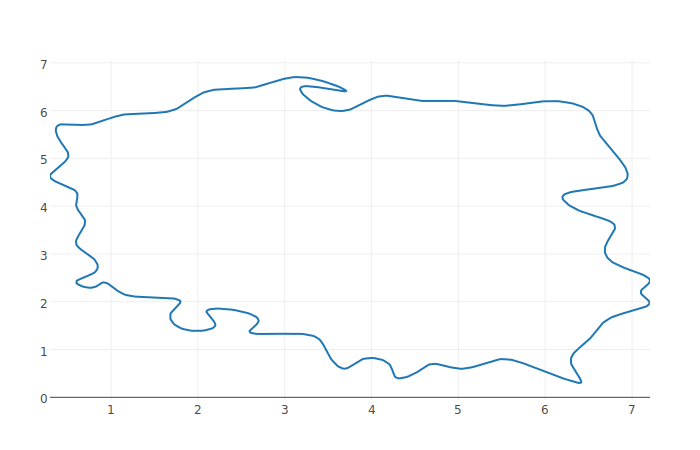
\includegraphics[width=0.8\textwidth]{poland}
    \caption{Interpolacja tajemniczej krzywej}
    \label{fig:poland}
\end{figure}

\begin{figure}[h]
    \centering
    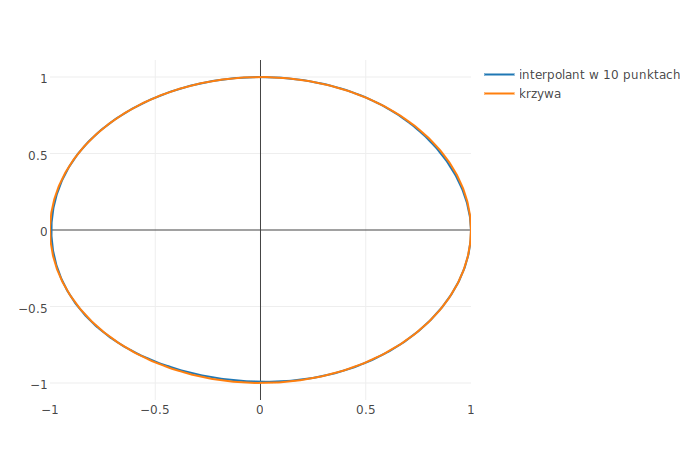
\includegraphics[width=0.8\textwidth]{circle}
    \caption{Interpolacja koła}
    \label{fig:poland}
\end{figure}

\begin{figure}[h]
    \centering
    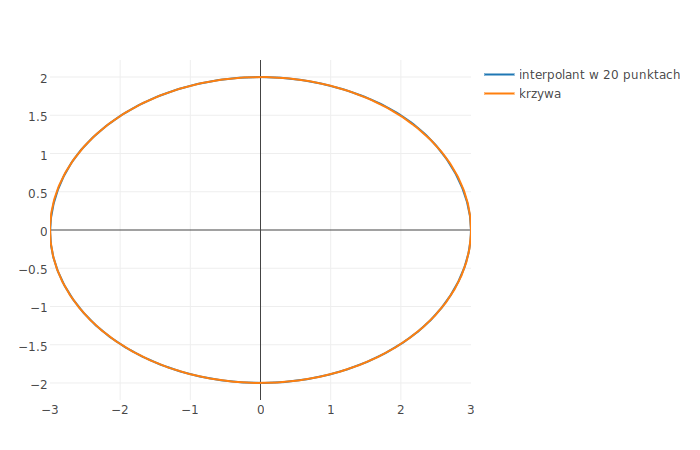
\includegraphics[width=0.8\textwidth]{ellipse}
    \caption{Interpolacja elipsy}
    \label{fig:ellipse}
\end{figure}

\begin{figure}[h]
    \centering
    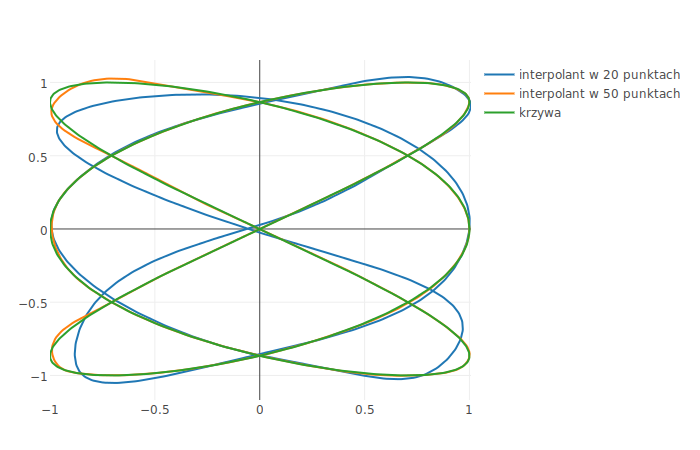
\includegraphics[width=0.8\textwidth]{lissajous}
    \caption{Interpolacja krzywej Lissajous dla 20 i 50 punktów interpolacyjnych}
    \label{fig:lissajous}
\end{figure}

\begin{figure}[h]
    \centering
    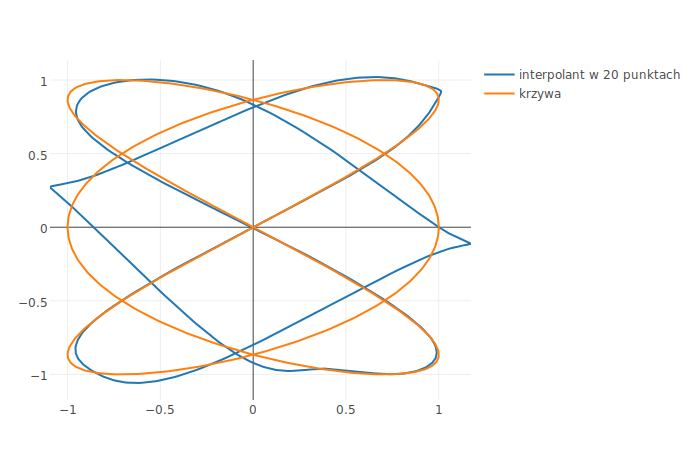
\includegraphics[width=0.8\textwidth]{equidistant}
    \caption{Interpolacja krzywej Lissajous, paramteryzacja równoodległa}
    \label{fig:equidistant}
\end{figure}

\begin{figure}[h]
    \centering
    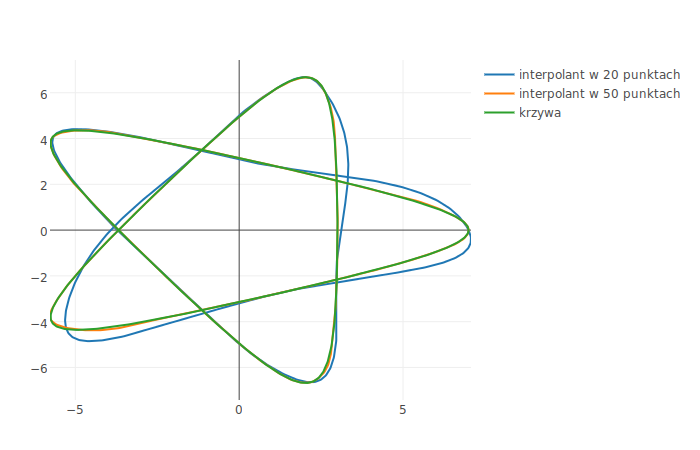
\includegraphics[width=0.8\textwidth]{hypotrochoid}
    \caption{Interpolacja hipotrochoidy  dla 20 i 50 punktów interpolacyjnych}
    \label{fig:hypotrochoid}
\end{figure}

\section{Analiza wyników i wnioski}

Jak widać na rysunku \ref{fig:ellipse} interpolacja krzywą sklejaną trzeciego stopnia pozwala na bardzo dokładne odwzoraowanie elips i okręgów, nawet jeśli danych jest niewiele punktów interpolacji. Dla bardziej skomplikowanych krzywych (rysunki \ref{fig:lissajous}, \ref{fig:hypotrochoid}) potrzeba już $ 50 $ punktów aby uzyskać kształt zbliżony do oryginału. Mimo tego, krzywa jest zawsze gładka, o ile korzystamy z kumulacyjnej strategii parametryzacji. Rysunek \ref{fig:equidistant} obrazuje problemy z parametryzacją równoodległą, która powoduje "kanty". Zjawisko to jest zbadane dokładnie w \cite{epstein}, gdzie autor udowadnia następujące twierdzenie.

\begin{tw}
	Jeżeli przebieg parametru $ t $ jest wyznaczony za pomocą normy, to styczna do zamkniętej parametrycznej krzywej sklejanej trzeciego stopnia, interpolującej w punktach $ (t, x) $ oraz $ (t, y) $ będzie zmienna w sposób ciągły. 
\end{tw} 

Interpolacja funkcją sklejaną trzeciego stopnia pozwala na szybkie odtworzenie krzywej z niewielkiej ilości węzłów interpolacji. Korzystając z parametryzacji kumulacyjnej uzyskuje się krzywe które są zawsze gładkie i estetyczne. Warto pamiętać, że cały proces interpolacji ma złożoność liniową względem ilości punktów, także metoda ta jest szybka.

\section{Użycie programu}

Wszystkie funkcje dostępne są po wczytaniu pliku \texttt{program.jl}, najłatwiej testować procedurę interpolacyjną z pomocą procedury \texttt{test\_curve(curve, mode, ts)} której parametrami są
\begin{itemize}
\item \texttt{curve} - funkcja, która zaaplikowana do punktów próbkowania zwróci wektory $ x $ oraz $ y $
\item \texttt{mode} - strategia parametryzacji, \texttt{"cumulative"} lub \texttt{"equidistant"}
\item \texttt{ts} - punkty próbkowania
\end{itemize}
W kodzie źródłowym dostępne są krzywe Lissajous, elipsa, hipotrochoidy oraz tajemnicza krzywa. Wszystkie krzywe zaprezentowane są w zeszycie interaktywnym IJulia.

\begin{thebibliography}{99}

\bibitem{kincaid} David Kincaid, Ward Cheney, przekł.~Stefan Paszkowski,
\emph{Analiza numeryczna},
Warszawa, WNT, 2006.

\bibitem{dahlquist} Germund Dahlquist, \r{A}ke Bj\"{o}rck,
\emph{Numerical Methods in Scientific Computing Volume I}
SIAM, 2008

\bibitem{bjorck} \r{A}ke Bj\"{o}rck, Germund Dahlquist, przekł.~Stefan Paszkowski
\emph{Metody Numeryczne},
Warszawa, PWN, 1987

\bibitem{eigen} \r{A}ke Bj\"{o}rck, Gene H. Golub
\emph{Eigenproblems for Matrices Associated with Periodic Boundary Conditions}

\bibitem{epstein} M. P. Epstein, 
\emph{On the Influence of Parametrization in Parametric Interpolation},
SIAM Journal on Numerical Analysis Volume 13, Issue 2, 1976


\end{thebibliography}

\end{document}